\documentclass{sig-alternate-05-2015}

\usepackage{latexsym}
%\usepackage{acl2015}
\usepackage{url}
\usepackage[normalem]{ulem}	% Part of the standard distribution
\usepackage{multirow}
\usepackage[mathscr]{euscript}
\usepackage{graphicx}
\usepackage{enumitem}
%\usepackage{subfigure}
\usepackage{caption}
%\usepackage{subcaption}
\usepackage{color}
\usepackage{amsmath,amsfonts,amssymb}
\newcommand{\red}[1]{\textcolor{red}{#1}}
\newcommand{\ignore}[1]{}

\usepackage{floatrow}
% Table float box with bottom caption, box width adjusted to content
\newfloatcommand{capbtabbox}{table}[][\FBwidth]

\usepackage{blindtext}

\begin{document}
\setcopyright{acmcopyright}
% DOI
\doi{10.475/123_4}

% ISBN
\isbn{123-4567-24-567/08/06}

%Conference

\acmPrice{\$15.00}

%
% --- Author Metadata here ---
\conferenceinfo{SIGIR}{'16 San Francisco, Californoa USA}
%\CopyrightYear{2007} % Allows default copyright year (20XX) to be over-ridden - IF NEED BE.
%\crdata{0-12345-67-8/90/01}  % Allows default copyright data (0-89791-88-6/97/05) to be over-ridden - IF NEED BE.
% --- End of Author Metadata ---

\title{Learning to Translate for Multilingual Question Answering}

\numberofauthors{1} %  in this sample file, there are a *total*


\author{
(Blinded for reviews)
%\alignauthor
%Ferhan Ture\\
%\affaddr{Raytheon BBN Technologies}\\
%\affaddr{10 Moulton St. Cambridge, MA 02138}
%\email{fture@bbn.com}
}
\date{}

\maketitle
\ignore{
\begin{abstract}

We introduce a machine learning-based approach for optimizing translation
in multilingual question answering (MLQA). In MLQA, there are multiple methods
to translate the question and/or answers, four of which we explore in this paper. We 
build a feature for each combination of translation \emph{direction} and \emph{method}, 
and train a model that learns optimal feature weights.
%Using this model to rank answers is statistically 
%significantly better translating all text into English. 
On a large multilingual forum,
our novel \emph{learn-to-translate} approach was more effective than a typical
MLQA approach ($p<0.05$):\ translating all text into English, then training 
a classifier based only on English (original or translated) text.
%\red{Baseline = 1-best translation of question into doc language. Cosine similarity between tf-idf vectors representing
%question and document, both in doc language.}


%%The World Wide Web is expanding and evolving into a vast network of less structured, more informal, multilingual, and diverse data. 
%This paper presents an approach for question answering (QA) in multilingual collections.
%%that attempts to address the multilingual and informal aspect of the Web. 
%We incorporated the multilingual aspect into our answer ranking models in two ways:\
%First, we introduced novel bilingual features based on a two-way probabilistic translation of 
%both questions and answers. Second, we filtered available training data based on language-related criteria.
%In addition to improvements in modeling, we also explored a more language-aware approach, 
%by building multiple language-specific answer ranking models, and merging the answers.
%%also implemented language-specific answer ranking and compared two approaches for applying these classifiers to multilingual QA.
%%One approach uses a single classifier to score all question-answer pairs (regardless of language), while the other applies 
%%a separate custom classifier for each language in the collection -- in the latter case, answers are merged in the final stage. 
%%Experiments were conducted on the DARPA BOLT task, consisting of a collection of Arabic, Chinese, and English Web forum 
%%posts, and a set of complex non-factoid questions expressed in English. 
%Experiments on a large collection of forum threads revealed that
%%we present valuable empirical results on the design and implementation of multilingual QA 
%%systems. In two out of the three tasks that retrieve non-English answers, results show that 
%%we show the effectiveness of our answer ranking model:\ 
%our novel answer ranking model 
%%including bilingual features and 
%%selecting data based on language 
%yields statistically significant improvements. 
%While using multiple classifiers did not yield the expected increase in overall effectiveness, we present 
%arguments for further exploration of this framework.
%% for ranking answers in multilingual collections
%%that deserves further exploration.

%\vspace{1mm}
%\noindent
%{\bf Categories and Subject Descriptors}:\ H.3.3 {[Information Storage
%    and Retrieval]}:\ Information Search and Retrieval
%
%\vspace{1mm}
%\noindent
%{\bf General Terms:} Algorithms, Experimentation
%
%\vspace{1mm}
%\noindent
%{\bf Keywords:} multilingual data, question answering, clqa
\end{abstract}
}

\section{Introduction}
%General task definition: finding answers to a posed question from user in their own language. answers might come from any language.

%Motivation: importance of approaches that can handle multilingual data.
%\vspace{-0.2cm}
%\paragraph{Motivation}
%As the World Wide Web is expanding, it is also evolving:\ social media is used more extensively and diversely; access to internet has 
%increased, especially in less developed countries; and smartphone use has increased exponentially. Over the years, all of these factors 
%have transformed the Web from an English-centric, mostly academic and formal network into a vast network of less structured, more informal, 
%more social, more multilingual, and more diverse data. As a result, Web search has become more challenging, requiring efficient and effective 
%natural language processing (NLP) tools for success.
%The same factors that make Web search challenging have also turned it into a more interesting task. 
%Retrieving information from the Web can be part of many potential applications in domains such as political analysis, social studies, military
% intelligence, as well as popular mobile platforms that help users find relevant information immediately. 
%Question Answering (QA) is one way to search the Web for relevant information -- it allows a person to ask a natural-language question 
%(i.e., no special treatment, in their mother language) and receive relevant answers from the Web. Although research in QA has been 
%progressing for over a decade, the modern challenges of the Web motivate us to rethink how we have been approaching this problem and to 
%develop more robust and effective strategies.
%%\vspace{-0.5cm}
%\paragraph{Problem Description}

\emph{Question answering} (QA) usually consists of three stages: 
(a) preprocessing the question and collection, (b) retrieval of candidate answers in the collection, and (c) ranking answers with respect 
to their relevance to the question. The questions can range from factoid (e.g., ``What is the capital of France?") 
to causal (e.g., ``Why are trees green?"), and opinion questions 
(e.g., ``What do people think about lowering the drinking age in the United States?"). While earlier research has mostly focused on relatively 
simpler factoid questions, which have a single clear answer that can potentially be retrieved from a structured database, this is no longer 
a representative case in many real-world applications. 

%\red{ELABORATE MORE ON WHAT A NON-FACTOID QUESTION IS AND WHAT OUR APPROACH CAN AND CANNOT HANDLE}

%As stated above, the increasing usage of Internet and social media has transformed the task of QA; asking computers or mobile devices for 
%various types of information has become more prevalent, with more informal and possibly incomplete questions posed, and with broader data 
%sources available to search for answers. These changes have suggested that QA systems need to handle more sophisticated scenarios in a 
%more robust manner. For example, a journalist would like to be able to ask the system for people's opinions on a certain political event, which 
%would require a search through many online forum posts and to deal with many aspects of the topic, expressed in different languages
%and most likely in an informal way.

%While there is
%a lot of variety within each question type, it makes sense to construct approaches based on the type itself.
 
%In addition to the diversity of its content, the multilingual nature of the Web is another understudied aspect of QA. The amount of non-English 
%content on the Web is increasing faster than English; for example, one study\footnote{\url{http://www.internetworldstats.com/stats7.htm}} 
%reports that Arabic content is increasing an order of magnitude faster than English. 

\ignore{With more languages represented in the Web, 
QA systems (especially ones that use the Web as a data source) need to handle multilingual text effectively, even when the user is 
monolingual.}
The most common approach to \emph{multilingual QA} (MLQA) has been to translate all content into its most probable 
English translation via machine translation (MT) systems. This strong baseline, which we refer to as \emph{one-best MT} ({\tt 1MT}), has 
been successful in prior work~\cite{Adafre:2009aa,Hartrumpf:2009aa,Martinez-Gonzalez:2009aa,Lin:aa,Shima:2010aa}. 
However, recent advances in cross-lingual IR (CLIR) show that one can do better by representing the translation space 
as a probability distribution~\cite{Ture:2014aa}. In addition, MT systems perform substantially worse with user-generated text, such as web 
forums~\cite{Wees:2015aa}, which provides extra motivation to consider alternative translation approaches for higher recall.
To our knowledge, it has yet to be shown whether these recent advancements in CLIR transfer to MLQA.

%more sophisticated query translation methods produce significantly better results in the task 
%of cross-language IR.
%What if the candidate answers are in different languages? This is a realistic scenario, since web has more nonEnglish than English, with as many as X languages w
%ith over Y pages on the web.

We introduce a novel approach for MLQA, referred to as \emph{Learning to Translate} ({\tt L2T}), by developing a model that 
weights multiple translations of the question and/or candidate answer, based on how well it discriminates between good and bad answers.
%(with respect
%to a given question) by finding the optimal translation approach. 
Each translation of the question and/or answer is represented by a feature (Section~\ref{sec:repr}). The model then learns feature weights for 
each combination of translation \emph{direction} and \emph{method}, through a discriminative training process (Section~\ref{sec:feat}). 
In addition to our novel features, we also experimented with various data selection strategies to optimize model training (Section~\ref{sec:data}). 
Experiments conducted on the DARPA BOLT IR task\footnote{{\scriptsize \url{
http://www.darpa.mil/Our_Work/I2O/Programs/Broad_Operational_Language_Translation_(BOLT).aspx}}} 
confirm that our {\tt L2T} approach is statistically significantly better than {\tt 1MT} ($p<0.05$).
%in three out of four experiments. 


\textbf{Related Work:}
%\footnote{\url{http://trec.nist.gov}} 
%\footnote{\url{http://www.clef-initiative.eu}}
%\footnote{\url{http://research.nii.ac.jp/ntcir/index-en.html}}
Research in QA has mostly been driven by annual evaluation campaigns like TREC,%,\footnote{{\scriptsize \url{http://trec.nist.gov}}}
CLEF
%,\footnote{{\scriptsize \url{http://www.clef-initiative.eu}}} 
and NTCIR.
%\footnote{{\scriptsize \url{http://research.nii.ac.jp/ntcir/index-en.html}}} 
Most earlier work relied on either manually crafted rule-based approaches, or 
traditional IR-based approaches where each pair of question and candidate answer was scored using retrieval functions (e.g., 
BM25~\cite{Robertson:2004}). Alternatively, training a classifier for ranking candidate answers allows the exploitation of 
various features extracted from the question, candidate answer, and surrounding context~\cite{Madnani:2007aa,Zhang:2007aa}. 
In fact, an explicit comparison at 2007 TREC confirmed the superiority of machine learning-based approaches (F-measure 35.9\%
vs 38.7\%)~\cite{Zhang:2007aa}. Learning-to-rank approaches have also been applied to QA successfully~\cite{Agarwal:2012aa}.
%Especially following the success of IBM's Watson QA system~\cite{Ferrucci:2010aa} on ``Jeopardy!'', there has been increased
%popularity in building complex QA systems that learn from large amounts of structured and unstructured data. Microsoft, 
%Facebook and many other technology companies are investing in deeper learning approaches to QA~\cite{Wang:2014aa,Bordes:2014aa}.

\ignore{Previous ML-based approaches have introduced useful features from many aspects of natural language, 
including lexical, syntactic, semantic, and discourse features. Surface text can indicate answer relevance; converting the surface 
text of the question and answer into a bag-of-words vector allows one to quantify textual similarity~\cite{Brill:2001aa}. 
Expanding the surface text with synonyms and other related concepts increases robustness~(e.g., \cite{Attardi:2001aa}).
% => boolean or frequency-weighted vector space model.
Syntactic analysis can reveal deeper relationships between the question and answer pair~\cite{Katz:2003aa}.
Detecting the part-of-speech tags, identifying indicative noun and verb phrases, and extracting the parse
tree can yield useful cues in QA~\cite{Alfonseca:2001aa,Katz:2005aa}.
Ideally, we would like to match meaning instead of raw text, and analyzing
various semantic aspects of language is beneficial~\cite{Cui:2005aa,Katz:2005aa,Alfonseca:2001aa,Hovy:2001aa}.	
}
% has proven to improve QA performance significantly
%Predicting the expected answer type~\cite{Harabagiu:2000aa,Moldovan:2007aa,Zhang:2003aa}
%has been very useful for factoid-type questions; for non-factoid questions, Chaturvedi et al. have explored representing
%the question type as a latent variable~\cite{Chaturvedi:2014aa}. There has also been work that classifies
%questions as factoid or non-factoid before processing~\cite{Aikawa:2011aa}.

\ignore{Additionally, semantic role labeling and dependency trees are other forms of semantic analysis used widely in NLP
applications~\cite{Shen:2007aa,Cui:2005aa}.
When searching for answers in text, humans mostly consider the surrounding context, often referred to as \emph{discourse}.
Researchers have explored certain ways to extract useful information from the adjacent sentences or even the entire document,
such as coreference resolution~\cite{Morton:1999aa}, or identifying temporal/spatial references~\cite{Saquete:2005aa,Harabagiu:2005aa},
which are especially useful for ``why'' and ``how'' questions~\cite{Kolomiyets:2011aa}.
}
%Why questions are studied by Verberne et al. [141]. How questions are investigated in [9]. On the recognition of rhetorical 
%relations in expository texts, the work of [75] is very relevant. Recent advances in text-based argumentation detection [104] 
%open up new research avenues for answering Why questions"

%Other approaches include the use of structured data~\cite{Bilotti:2007aa,Severyn:2012aa} and logical representation and 
%reasoning~\cite{Moldovan:2007aa}, as well as treating QA as a textual entailment 
%problem~\cite{Harabagiu:2006aa,Mehdad:2010aa,Espla-Gomis:2012aa}.

When dealing with multilingual collections, most prior approaches translate all text into English beforehand, then
treat the task as monolingual retrieval (previously referred to as {\tt 1MT}). At recent 
evaluation campaigns like CLEF and NTCIR,\footnote{Most recent MLQA track was in 2008 for CLEF, and 2010 for 
NTCIR.} almost all teams simply obtained the one-best question translation, treating some online MT system as a black 
box~\cite{Adafre:2009aa,Hartrumpf:2009aa,Martinez-Gonzalez:2009aa,Lin:aa,Shima:2010aa}, with few notable 
exceptions that took term importance~\cite{Ren:aa}, or semantics~\cite{Munoz-Terol:2009aa} into account.
%Recent research in CLIR suggest that it is better to incorporate the translation space into the retrieval process.

\textbf{Contributions}: Ture and Lin recently described three methods for translating queries into the collection language 
in a probabilistic manner, improving \emph{document retrieval} effectiveness over a one-best translation 
approach~\cite{Ture:2014aa}.
Extending this idea to MLQA appears as a logical next step, yet most prior work
rely solely on one-best translation of questions or answers~\cite{Ko:2010ab,Garcia-Cumbreras:2012aa,Chaturvedi:2014aa},
or select the best translation out of few options~\cite{Sacaleanu:2008aa,Mitamura:2006aa}.
Mehdad et al. reported improvements by using a distance-based entailment score to choose among the top ten 
translations~\cite{Mehdad:2010aa}. 
%While Espla-Gomis et al. argue 
%that using MT as a black box is more convenient (and modular)~\cite{Espla-Gomis:2012aa}, there are potential 
%benefits from a closer integration between statistical MT and multilingual retrieval~\cite{Nie:2010}. 
To the best of 
our knowledge, there is no prior work where the \emph{\textbf{optimal query and/or answer translation is 
learned via machine learning}}.
In addition to learning the optimal translation, we show that \emph{\textbf{learning the optimal subset of the training data 
for a given task}} improves effectiveness. We select data based on either the source 
language of the sentence, or the annotation language. Such data selection strategies 
have not been studied extensively in the QA literature, therefore our results can provide useful insights to the community.
With these two contributions, we outperform the state of the art.

%CLEF'08 Multilingual QA track~\cite{Sacaleanu:2008aa,Adafre:2009aa,Hartrumpf:2009aa,Martinez-Gonzalez:2009aa,Munoz-Terol:2009aa}
%Adafre and Genabith: translate De q into En via BabelFish.
%Martinez-Gonzalez et al: translate Fr q into Es "with non-surprising poor results"
%Hartrumpf et al: translate En or Es q into De via Promt online MT service
%Sacaleanu et al: translate X to De via multiple online MT services (pick best by grammaticality). Replace NEs w/ placeholder before MT. Use En as interlingua if X-De MT not available.
%Munoz-Terol et al: translate En q to Es in two ways: translation of logic form (many heuristics, language-dep.), translation via MT. Latter works better.

%NTCIR-8 (2010)~\cite{Lin:aa,Ren:aa,Shima:2010aa}
%Lin and Kuo: translate En q into Ch via Google translate
%Ren et al: translate key terms in En q into Ch via Google/Yahoo translation engines with back-off to specialized bilingual dictionaries
%Shima and Mitamura: translate En q into Ja via Google translate
%<---- In all papers, these translation methods are used for document/candidate retrieval. The features for QA answer ranking system are always based on the translated text (no probabilistic representation, no multiple translations)

%EACL'06: Mitamura~\cite{Mitamura:2006aa} shows various methods to translate question for QA, but eventually selects one of the translations.

%Most of previous approaches focus on factoid question answering. Non-factoid questions have been relatively 
%under-explored, and dealing with them requires different strategies, since questions cannot be easily categorized via hand-crafted patterns that match question
%templates. This is true especially if the task is open-domain; the number of possibilities calls for a more learning-based approach
%that can take advantage of a diverse set of signals and can adapt to new domains. There is no perfect solution to this challenging
%task, but we are witnessing a surge of more sophisticated use of NLP to build more QA systems.

%TREC 2007 ciQA Task: University of Maryland
%
%http://trec.nist.gov/pubs/trec16/papers/umd.qa.final.pdf
%--> this is an approach where a classifier is trained to set weights of various features computed from the query and candidate answer~\cite{13880}.
%
%
%Michigan State University at the 2007 TREC ciQA Task
%
%http://trec.nist.gov/pubs/trec16/papers/michiganu.qa.final.pdf
%-- they use features from sentence, from query, from query-sentence pair
%-- train separate classifier for each query template
%-- baseline: no learning, just heuristics => classification-based approach superior.
%
%
%Joint Question Clustering and Relevance Prediction for Open Domain Non-Factoid Question Answering
%http://bit.ly/1G7PdrE
%
%-- Non-factoid questions are difficult to categorize into discrete types/templates (unlike factoid questions)
%     => baseline: predict the question category and use it explicitly during QA
%     => this work: model question type as a hidden variable
%-- Experiments on BOLT and TAC non-factoid task

% Kristen Patricia Parton, Columbia University
% Lost and Found in Translation: Cross-Lingual Question Answering with Result Translation
% This work Does not do sentence-level retrieval; they define CLQA as: document retrieval when query = question ///


%thread of work by Sanda Harabagiu and colleagues using this type of approach --- they look at it in terms of entailment or alternatively, paraphrase, e.g.,
%http://dl.acm.org/citation.cfm?id=1220289

%I don't know about cross-lingual, but for mono-lingual, look at:
%http://dl.acm.org/citation.cfm?id=1277802
%Where Matt applied ML techniques to a variety of rich features.


\section{Approach}\label{sec:main}

%In this section, we first give an overview of our approach, then dive into more details as we list four main hypotheses that guided our research.

Our work is focused on the \emph{answer ranking} stage of QA:\
%First, let us formally define the stage of the QA pipeline that we focus on throughout this paper, namely \emph{answer ranking}:\
Given a natural-language question $q$ in English, we score each $k$ candidate answers (either English, Arabic, or Chinese), 
in terms of its relevance to $q$. In our case, candidate answers are sentences extracted from all documents 
using the Indri retrieval engine~\cite{Metzler:2005}. 
%Hereafter, sentence and answer might be used interchangeably.
%While our approach is not language-specific, we assume (for simplicity) that questions are in English, whereas sentences are 
%in either English, Arabic, or Chinese. Non-English answers are translated back into English before 
%returning to user. 
%to the user in English, by translating back any non-English answer.
%As a preprocessing step, all non-English text snippets are translated into English.

\ignore{Our approach is not limited to any question type, factoid or non-factoid. Our main motivation is to provide good QA quality on
any multilingual Web collection. This entails finding answers to questions where there is no single answer, and for which human 
agreement is low.}

We aim to build a system that can successfully retrieve relevant information from open-domain and 
informal-language content. In this scenario, two common assumptions fail:\ i) we can accurately classify questions via template 
patterns (Chaturvedi et al. argue that this does not hold for non-factoid questions~\cite{Chaturvedi:2014aa})
and ii) we can accurately determine the relevance of an answer, based on its automatic translation into English (Wees et al. 
show how recall decreases when translating user-generated text~\cite{Wees:2015aa}).

Instead, we opted for a more adaptable approach, in which question-answer relevance is modeled 
using a discriminative classifier that represents a function of features intended to capture the relationship between the question 
and sentence text. We describe details throughout this section.
\ignore{
Instead of relying solely on a single potentially incorrect English translation, we increase our chances of 
a hit by translating both the question and the candidate answer, using four different translation methods.
Our main features, which are described throughout this section, are based on lexical similarity computed using these translations. 
The classifier is trained on a large number of question-answer pairs, each labeled by a human annotator with a 
binary relevance label.\footnote{Annotators score each answer from 1 to 5. We label any score of 3 or higher as relevant.} }
\ignore{We also show that restricting the classifier to a specific subset of training data can result in a much better model of relevance.}

%In our approach, we decided not to use template patterns to classify questions, since previous work suggests that it is difficult to 
%categorize non-factoid questions using such patterns.


%The rest of this section details our approach in the following order:\ representation of questions and answers (Section~\ref{sec:repr}), 
%classifier features (Section~\ref{sec:feat}), data selection (Section~\ref{sec:data}), and language-specific ranking 
%(Section~\ref{sec:oneclassperlang}).


%Given this overview, here are four hypotheses that guided our research:\\
%\underline{H1:} A bilingual view of the question-answer pairs can improve classification.\\
%\underline{H2:} Probabilistic translation of questions is more effective than one-best MT.\\
%\underline{H3:} Selecting a subset of training data based on language can produce a more effective classifier.\\
%\underline{H4:} It is better to train a custom classifier for each subtask (i.e., ranking answers from a specific language) and subsequently merge 
%language-specific answers into a mixed-language list.\\
%
%After describing our approach, we will test these hypotheses in the evaluation.
%While all of these hypotheses are intuitive, we are not aware of prior work for testing the validity of them.

% SOURCE-SIDE FEATURES

\subsection{Representation}\label{sec:repr}

%\paragraph{\red{Question vs Document Translation}}

In MLQA, since questions and answers are in different languages, most approaches translate both 
into an intermediary language (usually English). As a result, valuable information often gets ``lost in translation'', 
due to the error-prone nature of MT. These errors are especially noticeable when translating informal
text~\cite{Wees:2015aa}, or less-studied languages.

\textbf{Translation Direction}:
We perform a \emph{two-way translation} to better retain the original meaning:
%, and use that 
%information when modeling relevance (in addition to its translation).
%Based on this observation, 
in addition to translating each non-English sentence into English, 
we also translate the English questions into Arabic and Chinese (using multiple translation methods, described 
below). For each question-answer pair, we have two ``views'':\ comparing translated question to the 
original sentence (i.e., {\em collection-language} (CL) view); and comparing original question to the 
translated sentence (i.e., {\em question-language} (QL) view). 

%Our model then \emph{learns the most effective translation} direction and method by optimizing weights of the
%classifier, which we refer to as \emph{Learning to Translate}, and yields a more robust approach for question answering.
%Bidirectional translation allows the model to 
%predict (via training) the usefulness of each piece of evidence. 

\textbf{Translation Method}:
When translating text for retrieval tasks like QA, including a variety of alternative translations is as important as finding the most accurate 
translation, especially for non-factoid questions, where capturing (potentially multiple) underlying topics is essential.
%the objective is not to find the most accurate translation, since representing alternative
%translations can improve system recall. Instead, we aim to generate a more 
%complete picture of the translation space, without introducing too much noise. 
%Recent work in CLIR has shown that 
%incorporating probabilities from the internal representations of an MT system to ``translate'' the question can accomplish this, 
%outperforming the standard one-best translation~\cite{Ture:2014aa}. 
% due to a richer representation of the translation space
%We hypothesize that these improvements transfer to multilingual QA as well. 
We explored four \emph{translation methods} for translating
the English question into Arabic and Chinese. Each method outputs a probability distribution for 
each question word, expressing the translation space in the collection language:
%(details of first three methods can be found in \cite{Ture:2014aa}, fourth method is a slight
%variation of the lexical neural network translation model described in \cite{Devlin:2014}):}

%\begin{description}[topsep=0pt,itemsep=0ex,partopsep=1ex,parsep=1ex]

\noindent \underline{\emph{Word}}: In MT, a word alignment is a many-to-many mapping between source- and target-language words,
learned without supervision, at the beginning of the training pipeline~\cite{Och:2003a}.
These alignments can be converted into word translation probabilities~\cite{Darwish:2003aa}.
%In CLIR, it is common to compute word translation probabilities from word alignments~\cite{Darwish:2003aa}. \\
For example, in an English-Arabic parallel corpus, if an English word appears $m$ times in total and is aligned to a certain Arabic 
word $k$ times, we assign a probability of $\frac{k}{m}$ for this translation. This simple idea has performed greatly in IR for 
generating a probability distribution for query word translations.\\
\underline{\emph{Grammar}}: Probabilities can be derived from a synchronous context-free grammar, which is a typical
translation model found in MT systems~\cite{Ture:2014aa}. 
The grammar contains rules $r$ that follow the form {\tt $\alpha$ || $\beta$ || $\mathcal{A}$ || $\ell(r)$}, 
stating that source-language word $\alpha$ can be translated into target-language word $\beta$, with an associated likelihood value 
$\ell(r)$. $\mathcal{A}$ represents the word alignments.
For each rule $r$ that applies to the question text, we identify each source word $s_j$. From the word
alignment information included in the rule, we can find all target words that $s_j$ is aligned to.
By processing all the rules to accumulate likelihood values, we can construct translation probabilities for each word in the question.\\
\underline{\emph{10-best}}: Statistical MT systems can output a ranked list of translations, instead of the single best. 
Ture and Lin exploited this to obtain word translation probabilities from the top 10 translations of the question~\cite{Ture:2014aa}.\\
For each question word $w$, we can extract which grammar rules were used to produce the translation -- once we have the
rules, word alignments allow us to find all target-language words that $w$ translates into.
By doing this for each question translation, we construct a probability distribution that defines the translation space of each
question word.\\
\underline{\emph{Context}}: Neural network-based MT models learn context-dependent word translation probabilities -- 
the probability of a target word is dependent on the source word it aligns to, as well as a 5-word window of context~\cite{Devlin:2014}.\\
We modify the context-dependent lexical translation model from \cite{Devlin:2014} for question 
translation.  
However questions are sometimes not part of a full, well-formed sentence, so we randomly replace 
words in the window with a special filler token. This teaches the model how to accurately translate with full context, partial 
context, and no context.\\

%When comparing these methods, it is important to note that every method has its strengths 
%and weaknesses.
%; for example, the word-based translation generally provides many more translation alternatives (per word) than 
%the other methods, which might increase recall. On the other hand, it might also generate some noise due to its context-insensitive nature. 
%In contrast, the 10-best method lacks diversity compared to the word-based method (since the top 10 translations output by the MT system 
%are usually very similar), but can provide more accurate translations.
\vspace{-0.25cm}
For example, the question ``Tell me about child 
labor in Africa", which is simplified by our preprocessing engine to ``child labor in Africa", is translated into the following 
probabilistic structure:
% by \emph{grammar} translation.

%\begin{figure}[h!]
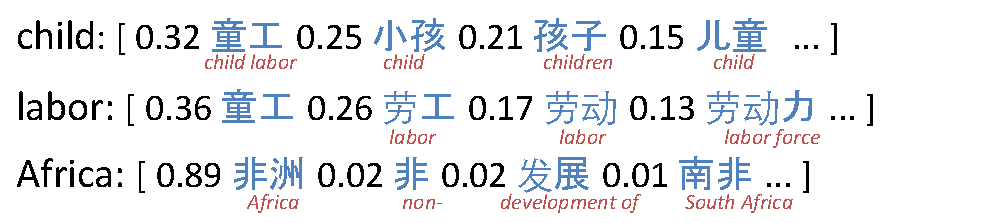
\includegraphics[width=7cm]{example.pdf}
%\caption{Probabilistic grammar-based translation of example question $q$ (call this $q_{\textrm{grammar}}$).}
% \label{fig:example} 
%\end{figure}

We are not aware of any other MLQA approach that represents the question-answer pair based on their probabilistic translation
space.
 
\subsection{Features}\label{sec:feat}

%\red{Since we have described how we implemented the bilingual view and how we probabilistically translate questions, we can now
%describe the feature set in detail}

Given two different translation directions (\emph{CL} and \emph{QL}), and four different translation methods (\emph{Word}, 
\emph{Grammar}, \emph{10-best}, \emph{Context}), our strategy is to leverage a machine learning process to determine how 
helpful each signal is with respect to the end task. For this, we introduced separate question-answer similarity features based 
on each combination of translation direction and method. 

%Each Arabic or Chinese sentence is converted 
%into a frequency vector, from which we compute the cosine similarity with each of the four query representations, resulting in four real-valued 
%lexical similarity features in the CL view (we call these {\tt LexCL}). 
Following figure shows how the probabilistic structure is converted into a single real-valued vector:
by averaging values for each Chinese word across the three distributions:
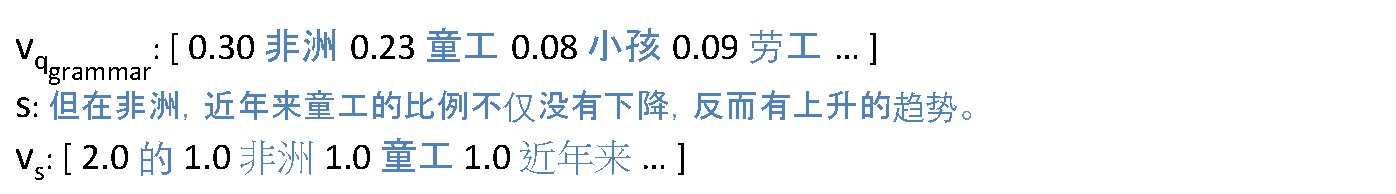
\includegraphics[width=7cm]{example2.pdf}

%shows how each English question word is represented by a probability distribution over the Chinese 
%vocabulary, using grammar translation. We convert this into a single real-valued vector by averaging values for each Chinese word across 
%the three distributions. 
Similarly, a candidate answer $s$ in Chinese is represented by scoring each word by its frequency. Given the two vectors, 
we compute the cosine similarity.
%:\ 
%$\sum_{\textrm{word }w} v_{q_{\textrm{grammar}}}(w) v_s(w) / |v_{q_{\textrm{grammar}}}| |v_s|$. 
The same process is repeated for the 
other three translation methods. These four lexical collection-language similarity features are collectively called \emph{LexCL}.
%, are shown in Figure~\ref{fig:features} and described in Table~\ref{tab:features}.
%\vspace{-0.3cm}
%\begin{figure}[h!]

%\caption{Vector representation of grammar-translated question ($q_{\textrm{grammar}}$) and sentence ($s$).}
% \label{fig:vector}
% \vspace{-0.2cm}
%\end{figure}
%\vspace{-0.2cm}

As mentioned before, we also obtain a similarity value by translating the sentence ($s_{\textrm{1best}}$) 
and computing the cosine similarity with the original question ($q$). Although it is possible to translate the 
sentence into English using the same four methods, we only used the one-best translation due to the computational 
cost. Hence, we have only one lexical similarity feature in the QL view (call \emph{LexQL}).
After computation, feature weights are learned via a maximum-entropy model.\footnote{We also 
tried support vector machines and noticed worse results.} We also include the 
same set of features from the previous sentence to represent the larger discourse.\red{A wider context did not
show further improvements in validation}

%For \emph{semantic similarity} features, we first parse the question $q$ (and translated sentence 
%$s_{\textrm{1best}}$), and then extract predicate-argument pairs into a \emph{text graph} $g_q$ 
%(and $g_{s_{\textrm{1best}}}$). Each node is an adjective, verb, noun, or proper name, 
%and the edges represent syntactic connections between them.
%% (like ``logical-subject'' or the preposition ``in'')
%We compute similarity between the $g_q$ and $g_{s_{\textrm{1best}}}$ in three ways:\ matching 
%the full tree, nodes, or edges~\cite{Freedman:2011aa}. Both nodes and edges can be matched entirely 
%or partially (e.g., via document co-reference or synonymy). These three features are called \emph{SemQL}, 
%since both graphs are represented in QL. 

%with some cost applied) to other nodes and edges
% Nodes and edges can also be dropped with some penalty.
%Similarity between the propositional tree of a question
%and a candidate answer can be computed in three different ways:\ matching the full tree, nodes, or edges~\cite{Freedman:2011aa}.
%\red{Add another sentence on how these values are computed.}

%While the quality of these features depend on the quality of linguistic resources (e.g., parser), we 
%compute the same features by translating the question into CL (call these three features \emph{SemCL}).
%The right side of Figure~\ref{fig:features} illustrates the computation process for the six features.

%it is still possible 
%to apply it to any language. Hence, we compute a set of semantic similarity features in both QL and CL (call \emph{SemQL} and 
%{\em SemCL}, respectively). 

%We only apply one-best translation for semantic similarity features, since it is not trivial to represent 
%the probabilistic translation in a graph.
%, we only apply
%one-best translation for semantic similarity features



%\begin{figure*}
%\begin{floatrow}
%\ffigbox{
%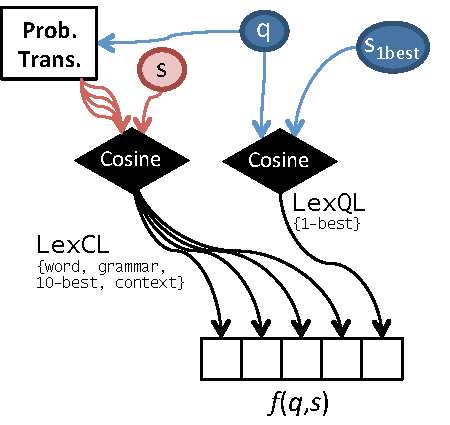
\includegraphics[width=5cm]{features.pdf}
%}
%{
%\caption{Feature computation process for an English question $q$ and non-English candidate answer $s$. 
%Light / dark oval nodes are in collection / question language, respectively. Nodes are duplicated to avoid crossing lines. 
%``Prob. Trans.'' generates the four probabilistic translations of $q$.}
%\label{fig:features}
%}
%%$s_{QL}$ and $q_{CL}$ represent the one-best translation of the sentence into QL, and the question into CL, respectively.
%\hspace{0.5cm}
%\capbtabbox{%
%\centering
%\begin{table}
%\begin{tabular}{|c|c|c|c|}
%\hline
%\textbf{Feature} & \# 	& \textbf{Question} & \textbf{Sentence} \\
%\textbf{category} & 	& \textbf{repr.} 	  & \textbf{repr.} 	    \\ \hline
%\multirow{4}{*}{LexCL} & 1 & $v_{q_\textrm{word}}$ & $v_s$\\\cline{2-4}
%				 & 2 & $v_{q_\textrm{10best}}$ & $v_s$  \\ \cline{2-4}
%				 & 3 & $v_{q_\textrm{context}}$ & $v_s$  \\ \cline{2-4}
%				 & 4 & $v_{q_\textrm{grammar}}$ & $v_s$  \\ \cline{1-4}
%LexQL 			& 5	& $v_q$ & $v_{s_\textrm{1best}}$   \\ \hline
%\multirow{3}{*}{SemCL} & 6 &  $g_{q_\textrm{1best}}$ & $g_s$ & full \\ \cline{2-5}
%				 & 7 & $g_{q_\textrm{1best}}$  & $g_s$ &  node \\ \cline{2-5}
%				 & 8 & $g_{q_\textrm{1best}}$  & $g_s$ &  edge \\\hline
%\multirow{3}{*}{SemQL} & 9 & $g_q$ & $g_{s_\textrm{1best}}$ & full  \\ \cline{2-5}
%				 & 10 & $g_q$ & $g_{s_\textrm{1best}}$ &  node \\ \cline{2-5}
%				 & 11 & $g_q$ & $g_{s_\textrm{1best}}$ & edge \\ \hline
%\end{tabular}
%\caption{List of features used in our QA system, where $v$ stands for the vector representation.}
%\label{tab:features}
%}
%{%
%  \caption{List of features used in our QA system, where $v$ stands for the vector representation.}%
%  \label{tab:features}
%}
%
%\end{floatrow}
%
%\end{figure*}
%\end{table}
% DATA SELECTION
\subsection{Data Selection} \label{sec:data}
There are at least two reasons why selecting training data based on language might benefit MLQA:\\
%\begin{enumerate}[topsep=0pt,partopsep=1ex]
i) Separating translation quality from relevance:\ If translation has errors, relevant answers might 
be judged as non-relevant. Training on this data might lead to a tendency to favor 
English answers higher than Arabic or Chinese.\\
ii) Filtering out noisy labels: 
%Answers extracted from non-English posts were annotated in one or both of two ways:\ 
%based on the original text, or based on its English translation (since the task requires returning answers in English). 
Since some pairs were annotated in both original language and English translation, independently, we can remove 
inconsistent ones from training.
%\item \underline{Improve learning:}\ Finally, from a purely ``machine learning'' perspective, it is always plausible that a certain 
%subset of the training data can produce a better model of relevance.
%\end{enumerate}

In order to explore further, we generated seven different subsets of the training set by filtering instances with respect to (i) the 
original \emph{language} of the answer, or (ii) the language of \emph{annotation} (i.e., based on original text or its
English translation):\\
\underline{\em lang=en}: Sentences from the English corpus.\\
\underline{\em  lang=ar/ch}: Sentences from the Arabic / Chinese corpus (regardless of how it was judged).\\
\underline{\em annot=consist}: All sentences except those that were judged inconsistently.\\
\underline{\em annot=src+}: Sentences judged only in original text, or judged in both consistently.\\
\underline{\em  annot=en+}: Sentences that are judged either only in English, or judged in both original and English translation consistently.\\
%\underline{\em all}: All sentences.
\vspace{-0.35cm}

% 1. Pipeline
% describe what we consider an answer (sentences split from documents), how we collect labeled data, what/how we train, how we score and rank (and any heuristics we apply).
% 2. Data selection
% why we care and how it relates to the multilinguality of the task
% list and describe various subsets

\section{Evaluation}\label{sec:eval}
In order to perform controlled experiments and gain more 
insights, we split our evaluation into four separate tasks:\ three tasks focus on retrieving answers from posts written in a specified language 
(\emph{English-only}, \emph{Arabic-only}, or \emph{Chinese-only}), and the last task is not restricted to any language 
(\emph{Mixed-language}). 

%Hypotheses H1, H2, and H3 were tested by comparing effectiveness under various classifier settings (changing the feature 
%set and training data). We repeated this for each task, since the effect might be task- or language-dependent. 
%Hypothesis H4 was tested by comparing the effectiveness of the two MLQA approaches described in Section~\ref{sec:oneclassperlang} 
%(\emph{L2T} and \emph{L2CT}).
%The rationale behind treating each separately is the hypothesis that 
%the classifier that works best for one task might not be optimal for another task.

All experiments were conducted on the IR evaluation task of the DARPA BOLT 
program. The collection consists of 12.6m Arabic, 7.5m Chinese, and 9.6m English Web forum posts, and a 
set of 45 non-factoid (mostly opinion and causal) English questions, all of which is preprocessed with 
sentence-splitting, named entity recognition, coreference resolution, parsing, and part-of-speech tagging. 
All non-English posts were translated into English, and all questions were translated into Arabic and Chinese,
using state-of-the-art English$\leftrightarrow$Arabic (En-Ar) and English$\leftrightarrow$Chinese 
(En-Ch) MT systems~[reference removed for anonymization]. 
The translation models were trained on parallel corpora from NIST OpenMT 2012, in addition to parallel forum 
data collected as part of the BOLT program (10m En-Ar words; 30m En-Ch words). 
From these data, word alignments were learned with GIZA++~\cite{Och:2003} (five iterations of IBM Models 1--4 
and HMM). While we only used the 
one-best English translation for sentences, we applied the probabilistic translation methods from Section~\ref{sec:repr} 
to questions. 
After all preprocessing, features were computed using the original post and question text, and their translations.
%, and the syntactic and semantic analysis output by our IE toolkit  
Training data were created by having annotators label all sentences of the top 200 documents retrieved per-question by Indri.
\ignore{
Due to the nature of retrieval tasks, labels of the training data are usually unbalanced, with more negatively labeled sentences. 
In order to correct this, we split the data into balanced subsets (each sharing the same set of positively labeled data) 
and train multiple classifiers, then take a majority vote when predicting.
}
%We later bootstrapped more candidate
%answers after rerunning the pipeline with a trained classifier. ==> no need to give details. In the end, we pretty much annotate all sentences in top 200 docs.

For testing, we froze the set of candidate answers and applied a trained classifier to each question-answer pair, generating
a ranked list of answers for each question. Evaluation was performed on this ranked list by computing average precision (AP). 
Due to the size and redundancy of the collections, we sometimes end 
up with over 1000 known relevant answers for a question. So it is neither reasonable nor meaningful to compute AP until we
reach 100\% recall (e.g., 11-point AP) for these cases. Instead, we computed AP-$k$, by accumulating precision values 
at every relevant answer until we get $k$ relevant answers.\footnote{$k$ was fixed to 20 in our evaluation, although we
verified that conclusions do not change with $k$ set to 50, 100, or 150.} %(we also tried 50, 100, and 150).
%\vspace{-0.2cm}

\textbf{Baseline}: As described earlier, the baseline system computes similarity between question text and the one-best 
translation of the candidate answer (we run the sentence through our state-of-the-art MT system). After translation, we 
compute similarity via scoring the match between the parse of the question text and the parse of the candidate answer, 
using our finely-tuned IE toolkit~[reference removed for anonymization].
%~\cite{Freedman:2011aa}. 
This results in three different similarity features:\ matching the tree node similarity, 
edge similarity, and full tree similarity. Feature weights are then learned by training this classifier discriminatively on the 
training data described above. This already performs competitively, outperforming the simpler baseline where we compute 
a single similarity score between question and translated text, and matching the performance of the recently 
published system by Chaturvedi et al on the BOLT evaluation~\cite{Chaturvedi:2014aa}. Baseline MAP values are 
reported on the leftmost column of Table~\ref{tab:controlled}.

%\red{How much weight did each feature get in classifier training?}
\textbf{Data effect}: In the baseline approach, we do not perform any data selection, and use all available data for training the
classifier. In order to test our hypothesis that selecting a linguistically-motivated subset of the training data
might help, we used 10-fold cross-validation to choose the optimal data set (among seven options described in 
Section~\ref{sec:data}). Results indicate that including English or Arabic sentences when training a classifier 
for Chinese-only QA is a bad idea, since effectiveness increases when restricted to Chinese sentences ({\tt lang=ch}).
On the other hand, for the remaining three tasks, the most effective training data set is {\tt annot=en+consist}.
These selections are consistent across all ten folds, and the difference is statistically significant for all but Arabic-only.
The second column in Table~\ref{tab:controlled} displays the MAP achieved when data selection is applied
before training the baseline model.

%In the lower part of Table~\ref{tab:controlled}, we reversed the scenario, by fixing the training data set, and using 
%10-fold cross-validation to select the optimal feature set. For the mixed-language and English-only tasks, best MAP is 
%achieved with the \emph{data set 7}. For Chinese-only QA, training on \emph{data set 4} yields statistically significant 
%improvements ($p<0.05$). Our findings support hypothesis H3 and suggest that the linguistic characteristics of data 
%deserves as much attention as its size -- specifically, we observed that including English or Arabic sentences when training 
%a classifier for Chinese-only QA is a bad idea; same can be said for including sentences that were annotated in 
%source-language only, when training a mixed-language classifier. 

\textbf{Feature effect}: In order to measure the impact of our novel features (Section~\ref{sec:feat}), we trained classifiers using either
\emph{LexCL}, \emph{LexQL}, or \emph{both} feature sets. In these experiments, the data is fixed to the
optimal subset found earlier. Results are summarized on left side of Table~\ref{tab:controlled}. Statistically
significants improvements over {\em Baseline} and {\em Baseline+Data selection} are indicated with single 
and double underlining, respectively.
 
%Given the strong baseline, we measured the effect of adding our
%features on top of \emph{SemQL}, considering all eight subsets of the remaining three feature categories. 
%For each feature set, we used 10-fold cross-validation to choose the optimal data set (among seven options described in 
%Section~\ref{sec:data}), as shown in the upper part of Table~\ref{tab:controlled}. 
For Arabic-only QA, adding \emph{LexQL} features yields greatest improvements over the baseline, 
while the same statement holds for \emph{LexCL} features for the Chinese-only task.
For the English-only and mixed-language tasks, the most significant increase in MAP is observed 
with all of our probabilistic bilingual features. For all but Arabic-only QA, the MAP is statistically significantly 
better ($p<0.05$) than the baseline; for Chinese-only and mixed-language tasks, it also outperforms baseline 
plus data selection ($p<0.05$).\footnote{Note that bilingual features are not expected to help on the 
English-only task, and the improvements come solely from data selection.}
%only base+LexQL did not create significant improvements over baseline, which was the only
%feature set without bilingual features. 
All of this indicates the effectiveness of our bilingual features and probabilistic question translation, 
as well as our data selection strategy.


%\setlength{\tabcolsep}{.25em}
\begin{table}[h]
\begin{small}
\centering
\begin{tabular}{|c|c|c|c|c|c|}
\hline
\multirow{2}{*}{\textbf{Task}} & \multicolumn{5}{|c|}{\textbf{L2T}}  \\ \cline{2-6}
	& \textbf{Baseline} & \multicolumn{2}{c|}{\textbf{+Data}} & \multicolumn{2}{c|}{\textbf{+Feats}}  \\ \hline
Arz & 0.421 & 0.423 & eng+ & { 0.425 } & LexQL   \\ \cline{1-6}
Cmn & 0.416 & \underline{0.425} & cmn-only & \underline{\underline{ 0.451 }} & LexCL  \\ \cline{1-6}
Eng & 0.637 & \underline{0.657} & eng+ & \underline{ 0.660 } & all  \\ \hline
Mixed & 0.665 & \underline{0.675} & eng+ & \underline{\underline{ 0.681} } & all \\ \hline
\end{tabular}
%\vspace{-0.2cm}
\caption{{\small Statistically significant increase over \emph{baseline} and \emph{+Data} are underlined 
(MAP with 10-fold cross-validation).}}
\label{tab:controlled}
\end{small}

\end{table}
%any_feat & 0.403 & 0.657 & 0.679 & 0.448\\ \hline

 
%\begin{table}[h]
%\begin{tabular}{lllll}
%Setting & Eng-only & Arz-only & Cmn-only & Mixed-lang \\
%Base    &          &          &          &            \\
%Best    &          &          &          &           
%\end{tabular}\label{tab:best}
%\end{table}

%While we notice that adding {\tt LexCL} features appear to have a positive effect in many cases, 

Understanding the contribution of each of the four \emph{LexCL} features is also important. To gain insight, we 
trained a classifier using all {\em LexCL} features (using the optimal data subset learned earlier for each task), and then 
incrementally removed one of the features, and tested on the same task. 
%selected the most-effective setting that included \emph{LexCL}:\ {\em feature set c} and {\em data set 1} 
%for Arabic-only task and (cmn-only data and ) for Chinese-only. We re-trained each 
%classifier four times, removing one of the \emph{LexCL} features each time, and tested on the same task. 
This controlled experiment revealed that the \emph{word} translation feature is most useful for Chinese-only 
QA (i.e., removing it produces largest drop in MAP, 0.6 points), whereas \emph{context} translation appears 
to be most useful (by a slighter margin) in Arabic-only QA. In the former case, the diversity provided by
word translation might be useful at increasing recall in retrieving Chinese answers. In retrieving Arabic
answers, using context to disambiguate the translation might be useful at increasing precision. This result
further emphasizes the importance of a customized translation approach for MLQA.

Furthermore, to test the effectiveness of the 
probabilistic translation approach (Section~\ref{sec:repr}), we replaced all {\em LexCL} features with a 
single lexical similarity feature computed from the one-best question translation. This resulted
in lower MAP:\ 0.427 to 0.423 for Arabic-only, and 0.451 to 0.425 for Chinese-only task ($p < 0.01$), 
supporting the hypothesis that \emph{probabilistic translation is more effective than the widely-used 
one-best translation}. In fact, almost all gains in Chinese-only QA seems to be coming from the
probabilistic translation.

To test the robustness of our approach, we let cross-validation select the best combination of 
(\emph{data}, \emph{feature}), mimicking a less controlled, real-world setting. In this case, the best 
MAP for the Arabic-only, Chinese-only, English-only, and Mixed-language tasks are 0.403, 0.448, 0.657, and 
0.679, respectively. In all but Arabic-only, these are statistically significantly better ($p < 0.05$) than 
not tuning the feature set or training data (i.e., Baseline). This result provides support that our approach
can be used for any MLQA task out of the box, and provide improvements.
%To summarize the results, we report the best MAP for each subtask in the left side of Table~\ref{tab:multiple}. 
%Right below MAP, the improvement over the baseline approach is shown for reference, with an asterisk mark if 
%statistically significant.

\section{Conclusions}\label{sec:concl}
%In this paper, we introduced novel bilingual features for multilingual QA, inspired from recent success in CLIR research.
%To our knowledge, this is the first use of probabilistic translation methods for this task, and the first attempt
%at using machine learning to learn the optimal translation approach for a given MLQA task. We described four 
%different methods to represent English questions in Arabic and Chinese vocabulary spaces, each of which adapts 
%various stages of modern statistical MT systems to translate questions more effectively.
%
%Additionally, we proposed using language-specific classifiers when ranking answers in a collection.
%Instead of assuming that ``one classifier fits all languages'', this approach treats the ranking of English, 
%Arabic, and Chinese answers as three separate subtasks, applying a separate classifier for each language.
%While post-retrieval merging has been studied in the past, we have not come across any work that applies this idea 
%specifically to create a language-aware ranking for MLQA.
%
%In order to provide an insightful analysis of our proposed approach, we set up an experimental evaluation to empirically 
%test various hypotheses.
%All experiments were conducted on the DARPA BOLT IR task, where the goal was to find
%relevant answers to 45 English non-factoid questions from a large collection of English, Arabic, and Chinese
%forum posts. This task represents a real-life scenario of searching through a diverse, informal, multilingual
%Web collection, with many challenges relevant to the QA research literature.

Our experimental analysis makes a strong case on how probabilistic
translation-based features and language-inspired data selection can improve QA effectiveness.
%Results did not support the hypothesis that learning a custom classifier for the retrieval of each language separately 
%would outperform the \emph{single classifier} baseline, but we still think that more research is needed to fully 
%understand how language-sensitive modeling can benefit MLQA. 
%For example, we would like to explore more sophisticated algorithms for merging multiple ranked
%lists of answers. Learning to rank between answers from different languages might be more effective than 
%heuristics. This would allow us to predict the final language ratio, based on many features (e.g., general
%collection statistics, quality of candidate answers, question category and complexity, MT system confidence levels) 
%to merge question-answer pairs.
An even more comprehensive use of machine learning would be to learn word-level translation scores, instead
of relying on translation probabilities from the bilingual dictionary, resulting in a fully customized translation
approach. Unlike monolingual IR~\cite{Bendersky:2010aa}, 
we are not aware of such an approach for multilingual retrieval. 
Another extension would be to apply the probabilistic translation methods for translating answers into
the question language (in addition to question translation). By doing this, we would capture the 
semantics of each answer much better, as one-best translation discards a lot of 
potentially useful information.

%Finally, since one of the take-away messages of our work is that a deeper understanding of linguistic context can 
%improve QA effectiveness via more sophisticated question translation, we are hoping to see even more improvements
%by creating features from deeper representations of text. Given the wide success of word embeddings, a possible
%next step is to learn bilingual embeddings for the task of QA, for which we have started adapting some related 
%work~\cite{Bai:2010aa}.


%\section{Acknowledgments}
%
%This research was supported in part by the BOLT program of the Defense
%Advanced Research Projects Agency, Contract No.\ HR0011-12-C-0015; NSF
%under awards IIS-0916043 and IIS-1144034. Any opinions, findings,
%conclusions, or recommendations expressed are those of
%the authors and do not necessarily reflect views of the sponsors. The
%second author is grateful to Esther and Kiri for their loving support
%and dedicates this work to Joshua and Jacob.

\bibliographystyle{abbrv}
\bibliography{qa}


\end{document}
